\section{Introduction}\label{sec:intro}

Despite the success of neural networks in various domains, their high inference cost
causes heavy burden on the environment and limits their deployment
in resource-constrained environments such as edge devices and IoT applications. 
A promising solution
is to learn Boolean networks (a special family of Boolean circuits, c.f. \cref{sec:background}) that operate directly on Boolean values, i.e., 0 and 1, instead of on floating-point numbers,
because 
Boolean operations are inherently more efficient in terms of computation, memory and power consumption.

A smaller Boolean circuit is generally cheaper to execute. 
For a given Boolean function, finding a compact,
or even minimal, Boolean circuit implementing this function is 
a fundamental and well-studied problem \citep{rudellMultipleValuedMinimizationPLA1987, ganai2000fly, micheli1994synthesis, bjesseDAGawareCircuitCompression2004,
 mishchenkoDAGawareAIGRewriting2006, rienerBooleanRewritingStrikes2022}. 
However, in practice, the Boolean function
is often not known a priori and must be learned from data. 

\paragraph{This Work: Learning Compact and Accurate Boolean Networks Efficiently}

We build on the learning framework proposed by \citet{petersen2022deep}. It works by
first relaxing a Boolean network into a differentiable representation and training it with gradient-based methods, 
and then discretizing it back into a Boolean network.
Despite existing efforts, three key challenges remain open. 
(i) \emph{Efficient connection learning}. 
\citet{petersen2022deep,petersen2024convolutional} and \citet{ruttgers2025light} randomly sample fixed connections between layers.
However, according to the lottery ticket hypothesis \citep{frankle2018the}, the ultra sparsity of Boolean networks (two inputs per neuron) makes random choices highly ineffective.
On the other hand, \citet{bacellar2024differentiable} and \citet{fojcik2025lilogic} 
parameterize the network connection with additional weight matrices, but this leads to significant memory and computational overhead during training, typically quadratic in the number of neurons per layer. 
(ii) \emph{Compact convolutional architecture}. The existing 
convolutional Boolean architecture \cite{petersen2024convolutional} utilizes 
a hardcoded tree-like kernel, which requires more Boolean operations (exponential in the depth of the tree) than a non-convolutional layer. 
(iii) \emph{Discretization-aware training}. The discrepancy between the differentiable relaxation and the discrete Boolean network causes
a clear accuracy drop after discretization.

In this paper, we address the aforementioned challenges and propose a novel method for 
learning compact Boolean networks. Our contributions are summarized as follows. 

\paragraph{Main Contributions}
\begin{itemize}
  \item We introduce a novel strategy to learn efficient connectivity for Boolean networks with no additional parameters and negligible computational overhead.
  \item We propose a compact convolutional Boolean architecture, removing hardcoded tree structures and reducing the number of Boolean operations.
  \item We develop an adaptive discretization strategy that progressively discretizes network layers during training, effectively reducing the discretization gap and improving final performance.
  \item Through extensive evaluation on vision benchmarks, we demonstrate that our method consistently learns more compact Boolean networks with higher accuracy (\cref{fig:acc_vs_gc}), achieving up to 37x fewer Boolean operations with better accuracy on \mnist when compared to \citet{petersen2024convolutional}, the prior state-of-the-art.
\end{itemize}

\begin{figure}
  \centering
  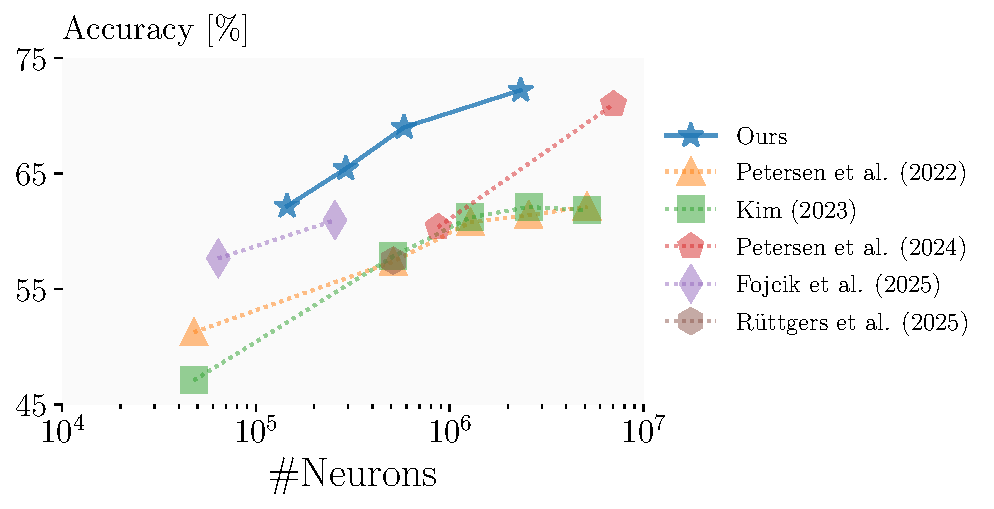
\includegraphics[width=.85\columnwidth]{figures/Acc_vs_GateCount.pdf} %
  \caption{Comparison between our method and prior works on \cifar. Note the log scale on x-axis.} \label{fig:acc_vs_gc}
  \vspace{-1em}
\end{figure}

The rest of the paper is organized as follows. 
\cref{sec:related_work} reviews the literature  
on  learning Boolean structures and 
reducing the inference cost of floating-point neural networks. 
\cref{sec:background} introduces the necessary background on learning Boolean networks via differentiable relaxations.
\cref{sec:method} and \cref{sec:experiments} presents and extensively evaluates our method, respectively.
Finally, \cref{sec:discussion} discusses the limitations and potential future directions.
